\setcounter{chapter}{2}
\chapter[\MakeUppercase{Kết quả mô phỏng, thực nghiệm hệ thống}]{Kết quả mô phỏng, thực nghiệm hệ thống}
Trong chương này, trước hết trình bày việc triển khai thuật toán MUSIC trên GNU Radio với dữ liệu giả lập từ Matlab để tránh các hạn chế của sóng vô tuyến như: nhiễu đa đường, phản xạ, nhiễu xạ, tán xạ gây khó khăn cho độ chính xác của thuật toán cũng như kiểm tra hoạt động của việc lập trình các khối OTT (Out Of Tree Modules) trên GNU Radio. Sau đó áp dụng trên các thiết bị SDR, phân tích các khó khăn và trình bày hướng giải quyết.

\section{Thực thi hệ thống dựa trên GNU Radio và dữ liệu giả lập từ Matlab}
\subsection{Mô tả dữ liệu mô phỏng}
Vẫn áp dụng mô hình tín hiệu như ở mục 1.2, các thông số mô phỏng như phía dưới:
{\renewcommand\labelitemi{}
\begin{itemize}
           \item $f = 914\textrm{ MHz}$                \hspace{1.6cm}\% Tần số
	\item $\lambda = c \div f = 0.328\textrm{ m}$	\hspace{0.4cm}\% Bước sóng
	\item $M = 4$				\hspace{2.88cm}\% Số phần tử anten của mảng thu
	\item $d = 0.5 \times \lambda$		\hspace{2.1cm}\% Khoảng cách giữa các phần tử anten mảng thu (\textbf{ULA})
	\item $D = 1$				\hspace{2.95cm}\% Số phần tử nguồn
	\item $angle = 85 \times (\pi \div 180)$ \% Góc tới của tín hiệu
	\item $gain = 0$				\hspace{2.5cm}\% Hệ số khuếch đại
	\item $SNR = 15\textrm{ dB}$			\hspace{1.5cm}\% Tỷ lệ tín hiệu tạp âm
	\item $k = 2 \times \pi \div \lambda$	\hspace{1.56cm}\% Hệ số sóng
	\item $K = 5000$				\hspace{2.3cm}\% Số mẫu thu thập
\end{itemize}
\begin{subequations}
\label{eq:all}
\begin{align}
\label{eq:model_a}
    \mathbf{s} &=
    \begin{bmatrix}
   	20^{\frac{SNR}{10}}\times \mathrm{randn}(1, K) + j \times \mathrm{randn}(1, K)
    \end{bmatrix}\\
\label{eq:model_b}
    \mathbf{A} &=
    \begin{bmatrix}
	10^{\frac{gain}{10}} \times \mathrm{exp}\{j \times k \times (0:M-1) \times d \times \cos(angle)\}
    \end{bmatrix}^T \\
\label{eq:model_c}
 \mathbf{n} &=
    \begin{bmatrix}
	\mathrm{randn}(M, K) + j \times \mathrm{randn}(M, K)
    \end{bmatrix} \\
\label{eq:model_d}
 \mathbf{x} &=
    \begin{bmatrix}
	\mathbf{A}\mathbf{s} + \mathbf{n}
    \end{bmatrix}
%\end{equation} 
\end{align}
\end{subequations}

Sử dụng Matlab tạo mô phỏng dữ liệu đầu vào với những thông số như trên, thu được được ma trận $\mathbf{x}(t) \in \mathbb{C}^{4 \times 5000}$, lưu trữ nó vào file \textit{source.mat} bằng hàm có sẵn của Matlab. Việc tiếp theo là đưa dữ liệu mô phỏng vào GNU Radio, dưới đây là phương pháp tạo khối để nhận vào dữ liệu mô phỏng và khối tính toán, hiển thị DOA cho người dùng.

\subsection{Sơ đồ khối và mô tả sơ đồ khối}

Đối với mục đích mô phỏng trong phần này, Synchronous Blocks được sử dụng: 1 khối loại bỏ đầu vào và thay thế bằng file dữ liệu mô phỏng tử Matlab tạo thành khối nguồn; 1 khối loại bỏ đầu ra tạo thành khối đích để tính toán và hiển thị giao diện DOA. Sử dụng Pỵthon để tiết kiệm thời gian viết khối, sơ đồ khối của việc mô phỏng thực hiện như hình \ref{fig:simulation}.

\begin{figure} [h]
	\centering
	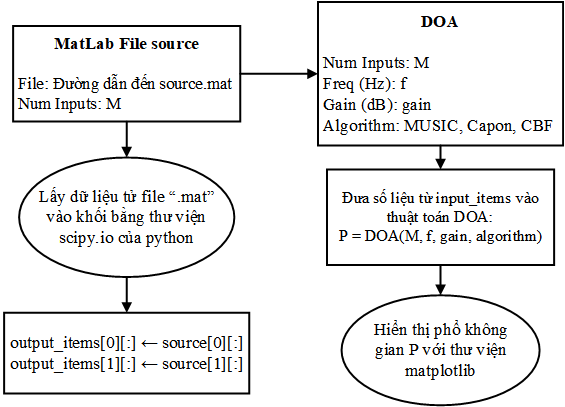
\includegraphics[width=0.9\linewidth]{figures/simulation.png}
	\caption{Sơ đồ làm việc DOA với dữ liệu mô phỏng Matlab}
	\label{fig:simulation}
\end{figure}

\subsection{Kết quả thực thi và đánh giá}

Lập trình khối theo sơ đồ khối \ref{fig:simulation}, cài đặt và tích hợp chúng vào GNU Radio, liên kết 2 khối, kết quả như hình \ref{fig:simulation1}.

\begin{figure} [!hb]
	\centering
	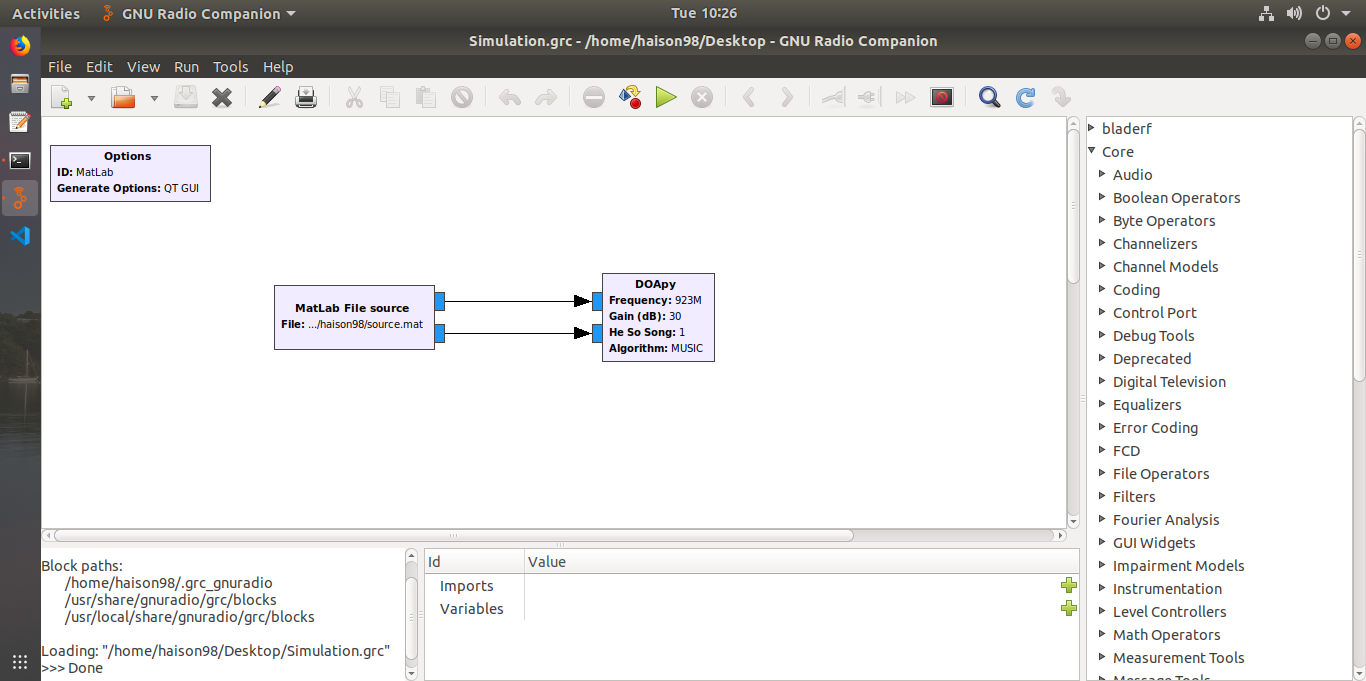
\includegraphics[width=1\linewidth]{figures/simulation1.png}
	\caption{Flow-graph ước lượng DOA với dữ liệu mô phỏng Matlab trên GNU Radio}
	\label{fig:simulation1}
\end{figure}

Nhập thông số đầu vào cho 2 khối và chạy chương trình. Kết quả thu được như hình \ref{fig:simulation2}.

\begin{figure}[h]
%\hfill
\subfigure[Kết quả của GNU Radio]{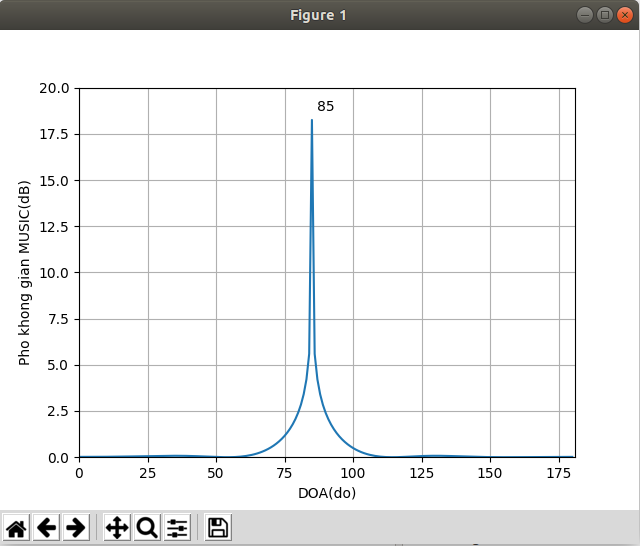
\includegraphics[width=0.49\linewidth]{figures/simulation3.png}}
\hfill
\subfigure[Kết quả của Matlab]{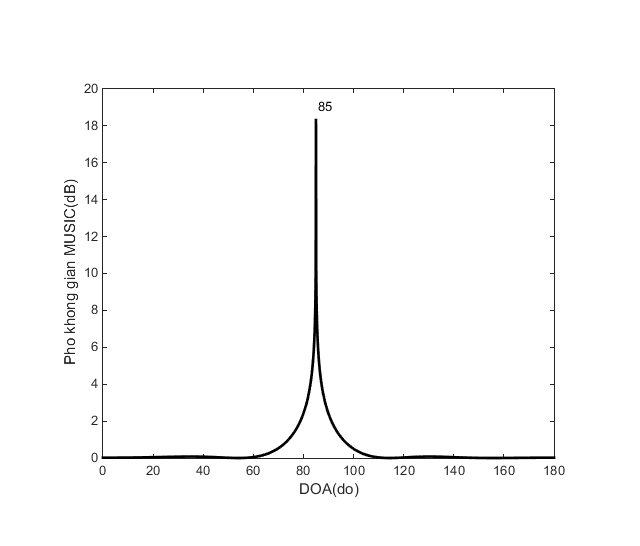
\includegraphics[width=0.49\linewidth]{figures/simulation4.png}}
\hfill
\caption{Kết quả ước lượng DOA với dữ liệu mô phỏng Matlab}
\label{fig:simulation2}
\end{figure}

Có thể thấy, với các thông số đầu vào lý tưởng, thuật toán chạy ổn định và đưa ra ước lượng DOA chính xác với mô phỏng trên Matlab trước đó. Đây là tiền đề để thực hiện hệ thống trên dữ liệu thực từ SDR.

\section{Thực thi hệ thống trên SDR với dữ liệu thực}

Sau khi đã mô phỏng thành công thuật toán trên GNU Radio với dữ liệu từ Matlab, bước tiếp theo là đưa BladeRF vào hệ thống để lấy dữ liệu thực tế. Tất nhiên từ việc sử dụng mô phỏng sang phần cứng sẽ gặp nhiều khó khăn hơn, tất cả sẽ được trình bày dưới đây.

\subsection{Tín hiệu nguồn phát}

Dữ liệu thực tế được dùng cho hệ tìm phương rất da dạng như: tín hiệu FM của các đài phát thanh, tín hiệu chuẩn DVB-T của đài truyền hình, GSM hay WiFi,... Dưới đây là 2 loại dữ liệu phổ biến âm thanh và video được điều chế và phát đi bằng BladeRF, được sử dụng như nguồn sóng đến cho hệ DOA.

NBFM: Điều chế NBFM trên GNU Radio với file nguồn là file âm thanh nén ở chuẩn WAV (Waveform Audio File Format).
\begin{figure} [!h]
	\centering
	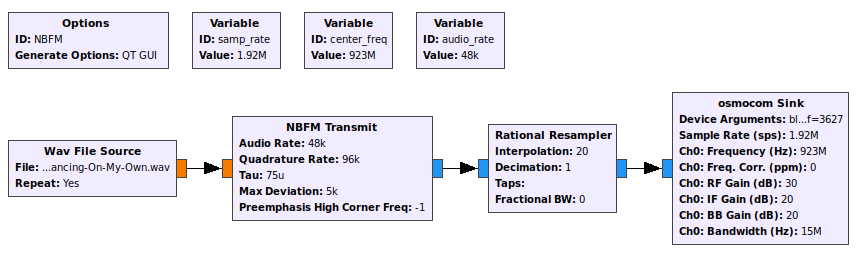
\includegraphics[width=0.9\linewidth]{figures/NBFM.png}
	\caption{Flow-graph truyền tín hiệu NBFM}
	\label{fig:NBFM}
\end{figure}

DVB-T: Điều chế chuẩn DVB-T trên GNU Radio với file nguồn là file video nén ở chuẩn TS (Transport Stream). Flow-graph bên dưới truyền video ở băng thông 8 MHz, chòm sao QPSK, tốc độ mã 7/8, khoảng bảo vệ 1/32, tốc độ lấy mẫu 10 MHz, tần số 923 MHz. Chi tiết hơn về việc sử dụng BladeRF truyền nhận DVB-T, DVB-T2 có tại \cite{BogdanDIA2015}.
\begin{figure} [!h]
	\centering
	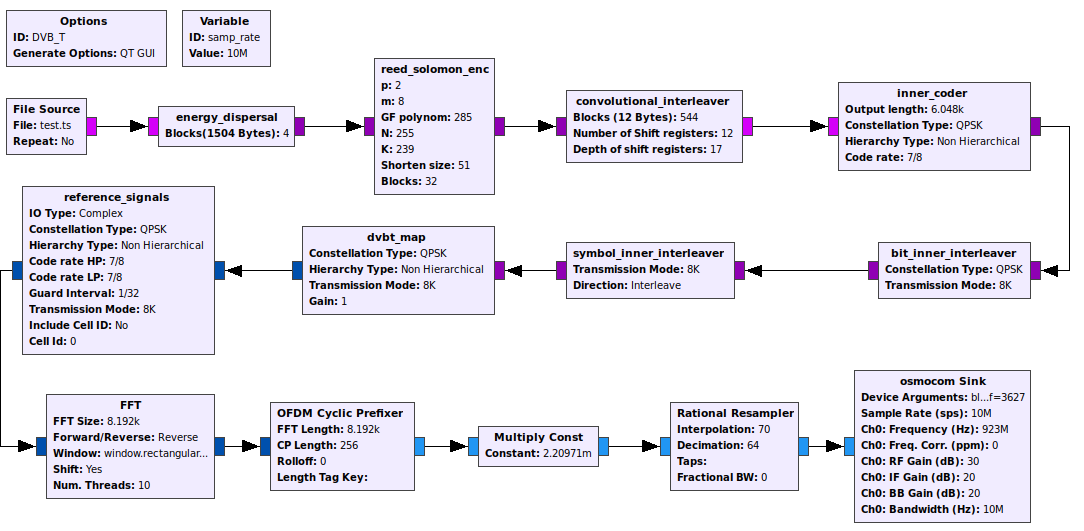
\includegraphics[width=0.95\linewidth]{figures/dvbt.png}
	\caption{Flow-graph truyền tín hiệu DVB-T}
	\label{fig:dvbt}
\end{figure}

\subsection{Sơ đồ khối và mô tả sơ đồ khối}

Các bước đồng bộ và ước lượng DOA được trình bày bên trên được kết hợp với nhau trên GNU Radio. Trước hết thực hiện các thiết lập trên \textit{bladerf-cli} như chia sẻ xung đồng hồ qua cổng SMB, hiệu chỉnh PPM của BladeRF. Sau đó sử dụng flow-graph trên hình \ref{fig:DoA_FM} phía dưới để đồng bộ và ước lượng DOA. Các khối tương ứng với chức năng chính:
\begin{itemize}
	\item Osmosdr Source: khối nguồn lấy dữ liệu trực tiếp từ các SDR, được phát triển dưới dạng mã nguồn mở,  hỗ trợ rất nhiều loại SDR: RTL-SDR, USRP, BladeRF, HackRF, LimeSDR, ... Có sẵn hầu hết các thông số đầu vào như tần số thu, tốc độ lấy mẫu, băng thông, khuếch đại,... tất cả đều trực quan và dễ dàng chỉnh sửa. %APIs
	\item DC Blocker: Loại bỏ thành phần 1 chiều trong tín hiệu.
	\item Low Pass Filter: bộ lọc thông thấp, dễ dàng chuyển đổi $f_\textrm{cut}$ tương ứng với trạng thái đồng bộ hoặc ước lượng DOA của hệ thống.
	\item Virtual Sink/Source: Các khối chuyển tiếp dữ liệu, giúp thu gọn và chia luồng dữ liệu để tiện xử lý.
	\item $\textrm{Sample}_\textrm{offset}$: Ước lượng mẫu offset do trễ đầu vào.
	\item PCA Phase Diff: Tính toán độ lệch pha giữa 2 tín hiệu cho bước đồng bộ SDR.
	\item Probe Signal/Funcion Probe: Lưu giá trị đầu vào dưới dạng biến làm thông số cho các khối khác.
	\item DOA/DOA Python: Khối ước lượng DOA được viết trên ngôn ngữ tương ứng C++/Python.
	\item QT GUI: Các khối hiển thị giao diện người dùng.
\end{itemize}
\afterpage{\clearpage}
\begin{figure} [!ht]
	\centering
	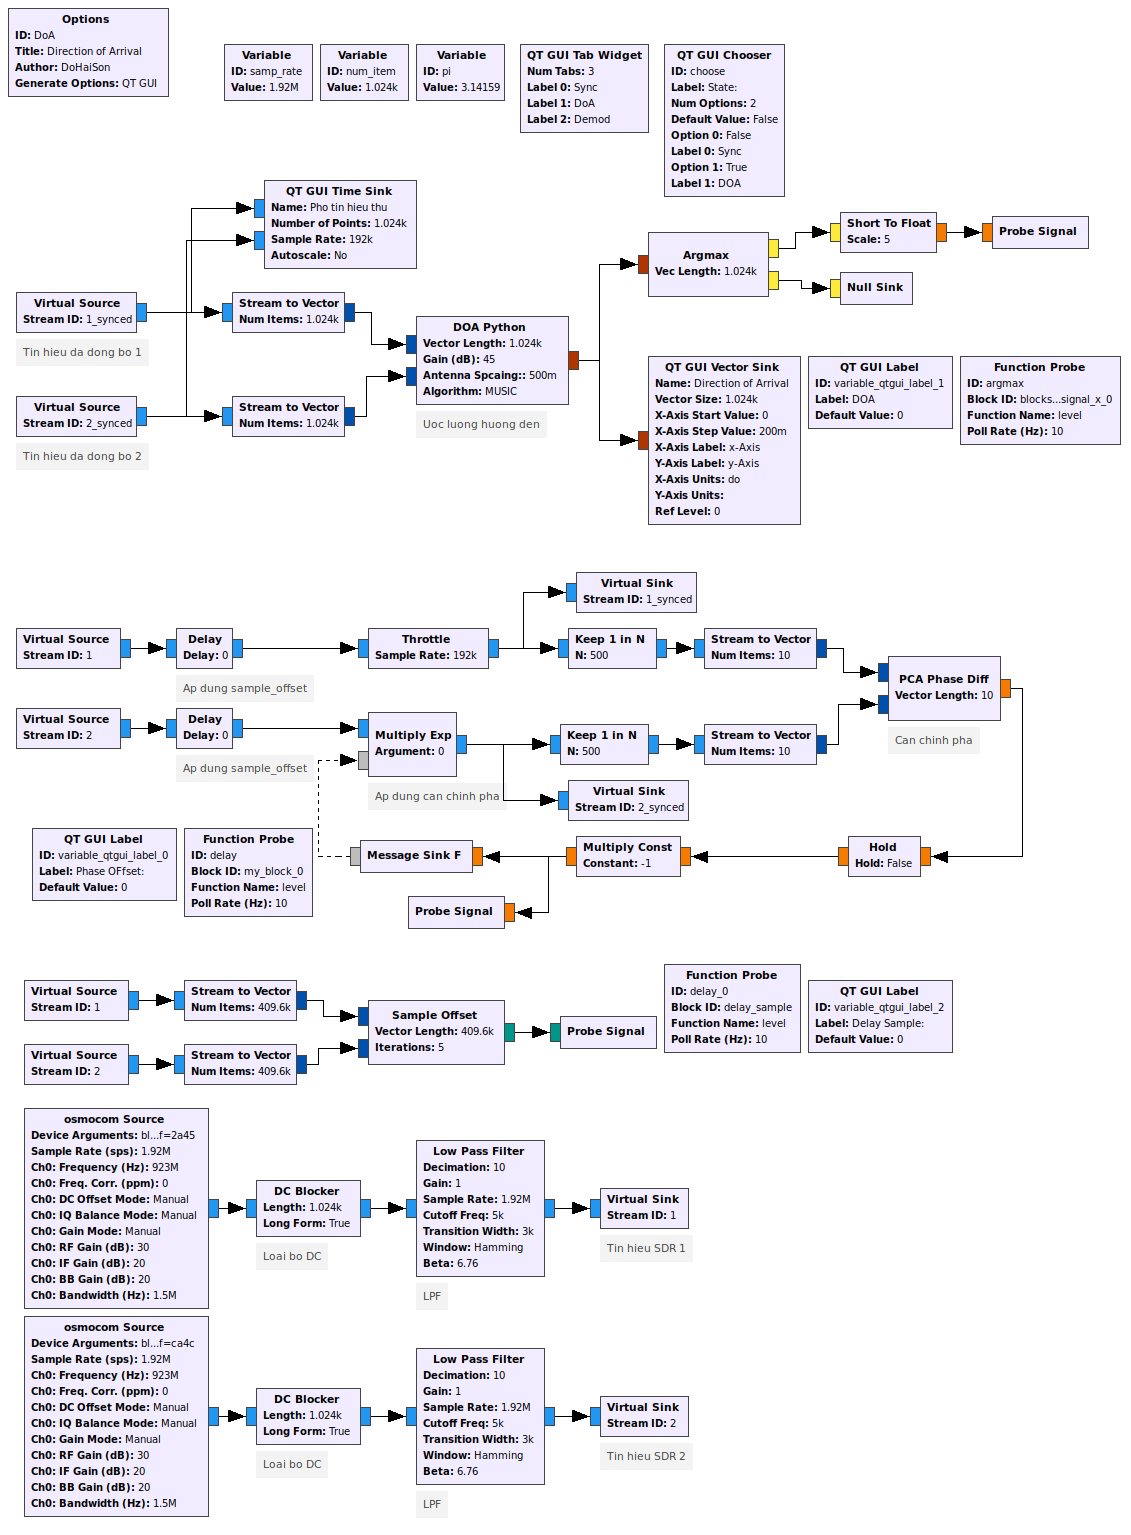
\includegraphics[width=\textwidth,height=\textheight,keepaspectratio]{figures/DoA_FM_grc.png}
	\caption{Flow-graph ước lượng DOA}
	\label{fig:DoA_FM}
\end{figure}
\newpage
\subsection{Kết quả thực thi và đánh giá}

Bố trí hệ thu phát sử dụng BladeRF để triển khai việc ước lượng phương tới trên BladeRF, trên hình \ref{fig:realsys} là hệ thống được cài đặt hoàn chỉnh, gồm 1 BladeRF phát và 2 BladeRF thu, cả 3 anten được sử dụng đều là anten không định hướng VERT2450. Cấu hình phần cứng và phần mềm của 2 máy tính thực hiện việc phát và thu trong dự án được nêu ra trong bảng \ref{table:hw}. Tần số được chọn là 923 MHz, là tần số nằm trong khoảng giữa của đường lên và xuống trong GSM900.
\begin{figure} [!h]
	\centering
	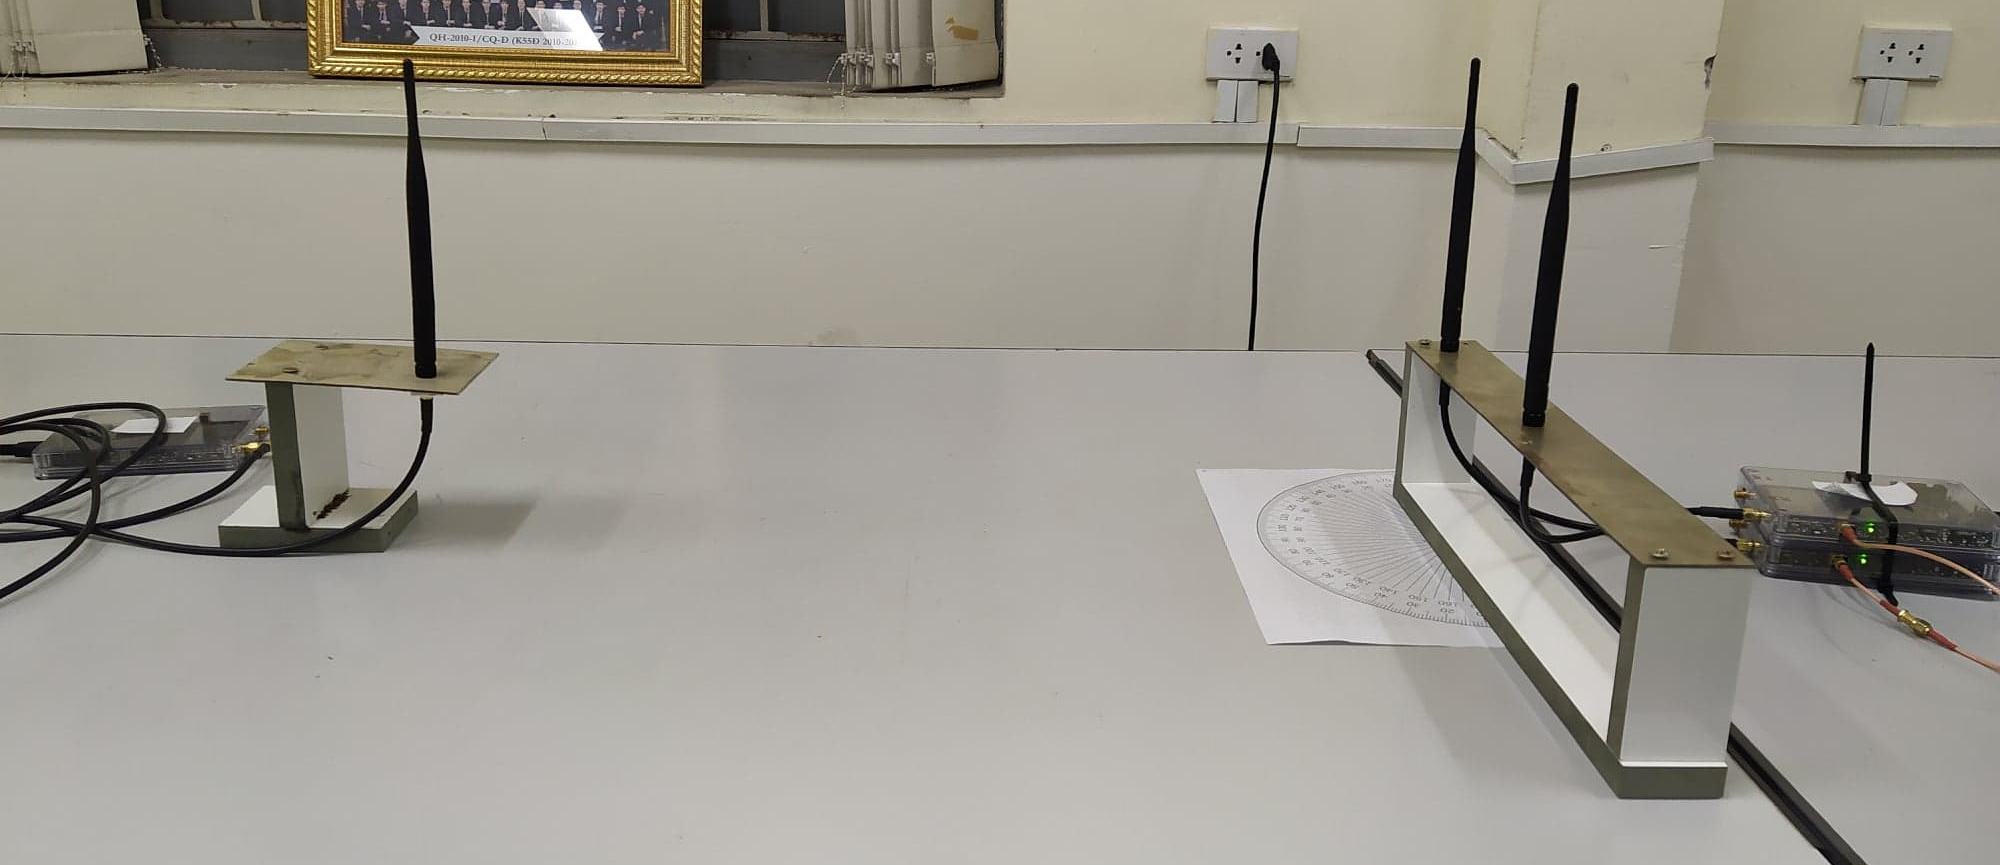
\includegraphics[width=1\linewidth]{figures/realsys.jpg}
	\caption{Sơ đồ bố trí hệ DOA thực}
	\label{fig:realsys}
\end{figure}
\begin{table}[!h]
\centering
\begin{tabular}{lcc}
\hline
\rowcolor[HTML]{FFE8E7} 
\multicolumn{1}{c}{\cellcolor[HTML]{FFE8E7}\textbf{Thông số}} & \textbf{Bên phát} & \textbf{Bên thu} \\ \hline
CPU & Intel Core I5-4800MQ & Intel Core I5-4210M \\
RAM & 8 GB & 8 GB \\
Hệ điều hành & Ubuntu 16.04 LTS & Ubuntu 18.04 LTS \\
Phiên bản GNU Radio & 3.7.11 & 3.7.11 \\ \hline
\end{tabular}
\caption{Thông số máy tính}
\label{table:hw}
\end{table}

Điều kiện thực nghiệm là phòng 204, nhà G2, Đại học Công Nghệ - Đại học Quốc Gia Hà Nội, tiến hành thực nghiệm 350 lần, xác định phương tới từ các góc khác nhau, để giảm thiểu sai số chủ quan độ phân giải khi thực nghiệm ở mức 5$^{\circ}$, bố trí hệ thống ở 3 vị trí khác nhau để đưa ra ảnh hưởng của môi trường đến độ chính xác của hệ DOA. Tín hiệu phát được thay đổi giữa DVB-T, NBFM.

Trong hình \ref{fig:dvbt_1} là kết quả sai số trung bình của hệ đặt DOA khi ở các vị trí khác nhau trong phòng, có thể nhận thấy, ở cả 3 vị trí thực nghiệm, khoảng góc từ 60$^{\circ}$ cho đến 140$^{\circ}$ đều cho sai số nhỏ dưới 6$^{\circ}$, đặc biệt ở các góc gần góc đồng bộ (90$^{\circ}$), độ sai số giảm xuống dưới 2$^{\circ}$. Điều này khớp với lý thuyết của hệ anten ULA, khi sai số sẽ tăng dần ở 2 biên của phổ công suất.

Tuy nhiên, cũng dễ dàng nhận thấy, sai số tăng dần ở 2 biên không đều như lý thuyết mà có khoảng tăng vọt như: 35$^{\circ}$ đến 60$^{\circ}$ ở vị trí 1; 135$^{\circ}$ đến 160$^{\circ}$ ở vị trí 2; 15 đến 40 ở vị trí 3. Những sai số này được tạo ra do nhiễu đa đường, do anten VERT2450 được sử dụng là anten không định hướng, vì vậy ở các vị trí xuất hiện vật cản, nhiễu đa đường sinh ra làm tăng tính tương quan của tín hiệu, và do thuật toán MUSIC yêu cầu không có sự tương quan giữa tín hiệu, kết quả thu được sẽ bị ảnh hưởng rất nhiều.
\begin{figure} [!h]
	\centering
	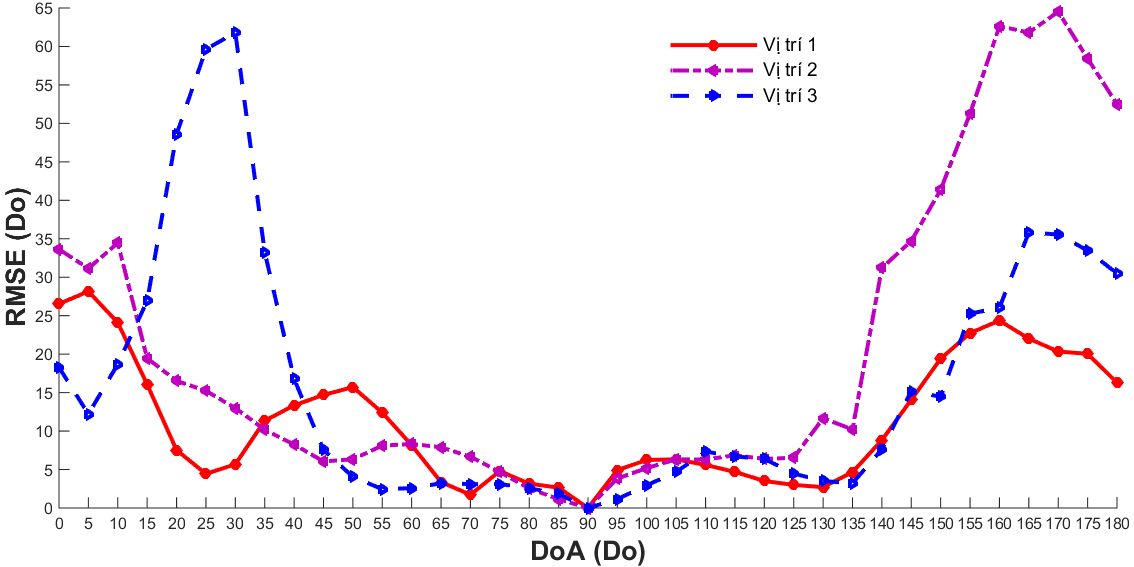
\includegraphics[width=1\linewidth]{figures/dvbt_1.png}
	\caption{RMS: Ở từng vị trí thực nghiệm}
	\label{fig:dvbt_1}
\end{figure}

Ngoài sai số thay đổi do vị trí hệ thay đổi, tín hiệu được sử dụng để đồng bộ hệ DOA và tín hiệu phát để xác định phương tới cũng ảnh hưởng tới kết quả đầu ra. Kết quả trên hình \ref{fig:dvbt_3} cho thấy, có sự giống nhau về sai số ở những góc xung quanh 90$^{\circ}$, nhưng với các góc ở xa, tín hiệu DVB-T lại cho kết quả tốt hơn.

NOTE: Trong thực nghiệm, theo em đo thì nếu đồng bộ bằng FM rồi chuyển sang DOA bằng loại tín hiệu khác, kqua sẽ dễ bị sai hơn. Còn DVB-T 64 QAM thì tương quan n thấp rồi, nên đồng bộ xong chuyển sang tín hiệu khác vẫn oke ạ.
\begin{figure} [!h]
	\centering
	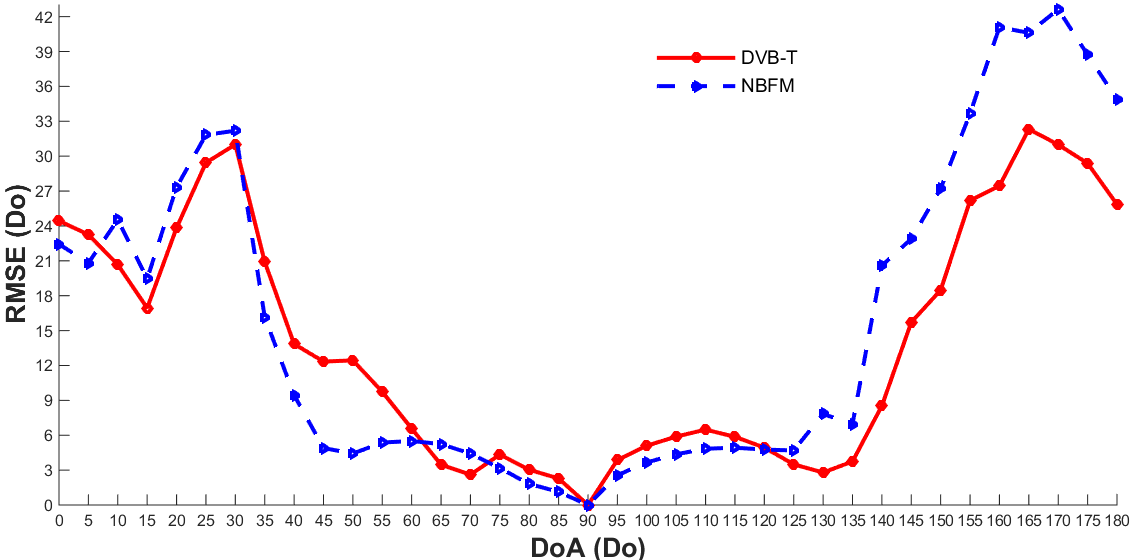
\includegraphics[width=1\linewidth]{figures/dvbt_3.png}
	\caption{RMS: DOA với tín hiệu NBFM và DVB-T}
	\label{fig:dvbt_3}
\end{figure}

Tổng hợp lại, hình \ref{fig:kqdoa} là kết quả trung bình của toàn bộ quá trình thực nghiệm với hệ DOA trên BladeRF, có thể thấy hệ giảm độ chính xác đáng kể khi góc tới ở ngoài khoảng 40$^{\circ}$ đến 140$^{\circ}$, do nhiễu đa đường, hay độ phân giải của mảng thấp do chỉ sử dụng 2 phần tử anten thu và bản chất của mảng anten ULA.
\begin{figure} [!h]
	\centering
	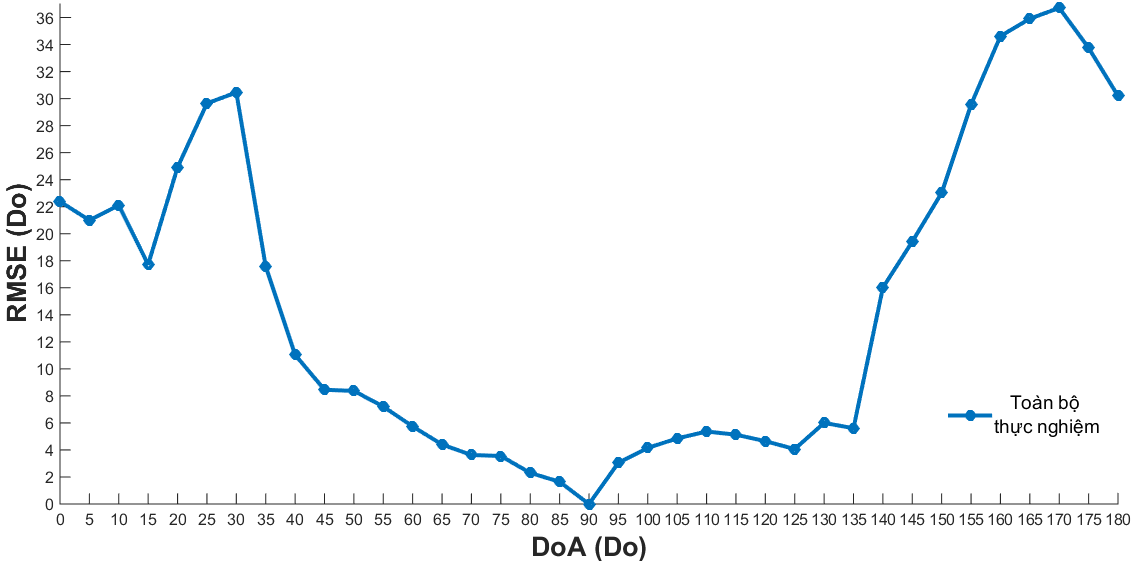
\includegraphics[width=1\linewidth]{figures/dvbt_2.png}
	\caption{RMS: DOA toàn bộ quá trình thực nghiệm}
	\label{fig:kqdoa}
\end{figure}
